\section{Latent Reasoning Path in Knowledge based Question Answering}\label{sec:2-2}

\subsection{Background}

Knowledge-based question answering (KBQA) is the task of finding answers to questions by processing a structured knowledge base $\mathcal{KB}$. %where the beliefs are stored as triples containing two entities and the relation linking them. 
A $\mathcal{KB}$ consists of a set of entities $\mathcal{E}$, a set of relations $\mathcal{R}$, and a set of literals $\mathcal{S}$. A knowledge base fact is defined as $(h,r,t)$, where $h\in \mathcal{E}$ is the head entity, $t \in \mathcal{E} \bigcup \mathcal{S}$ is the tail entity/literal, and $r\in \mathcal{R}$ is the directed relation between $h$ and $t$. To answer a simple single-relation question (\emph{i.e.} a 1-hop question) such as: \textit{``Who is the president of the United States?''}, a typical KBQA system first identifies the entity (\emph{i.e.} ``United States'') and the relation (\emph{i.e.} ``president'') asked in the question, and then searches for the answer entity by matching the entity-relation tuple <United States, president, ?> over $\mathcal{KB}$.

While a single-hop question can be answered by searching a predicate relation in $\mathcal{KB}$, it is much harder to answer more complex multi-hop questions containing multiple entities and relations with constraints. For complex questions, it is not easy to extract all the relations correctly together with their head and tail entities in the right order. Most prior work on multi-hop KBQA focus on learning a single given ground truth reasoning path for each question, and outputting the most possible reasoning path during prediction \cite{DBLP:conf/coling/ZhouHZ18,DBLP:journals/corr/abs-1801-09893,DBLP:conf/adbis/YuHYZW18,DBLP:conf/ijcai/LanW019}. However, it is common that $\mathcal{KB}$ has many alternative paths leading to the correct answer, of various reasoning qualities. These alternative reasoning paths are usually not provided as ground truth by the human annotators. Or there is no any labeled path in the given dataset at all, because in practice questions and answers are easy to collect (sometimes for free), but path annotation is very labor-intensive and expensive. 

\begin{figure}[t]
 \centering
 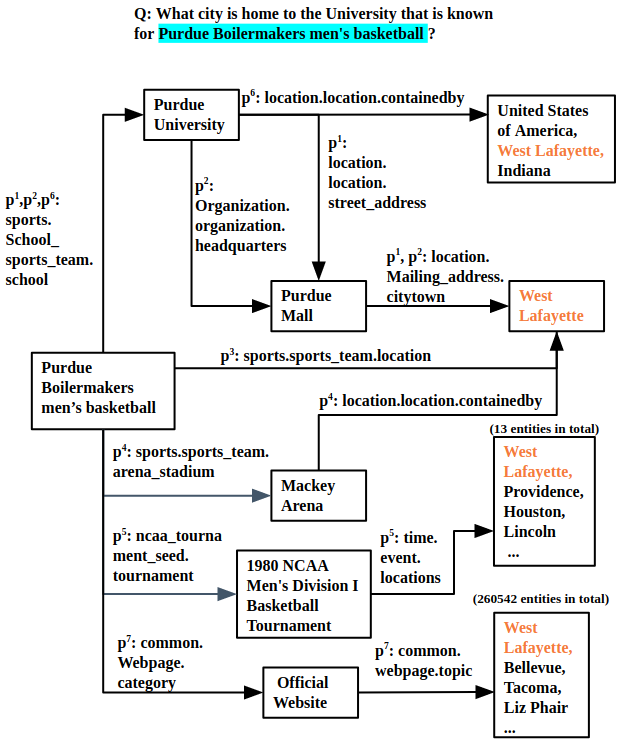
\includegraphics[width=0.7\linewidth]{Images/fig1.png}
 \caption{One QA example with Multiple Reasoning Paths from \textsc{ComplexWebQuestion}-1.1. The blue color highlighted is the extracted topic entity. Each square represents an entity, and the arrows represent the relations. Reasoning path $\mathbf{p}^1$ to $\mathbf{p}^4$ are the correct ones containing meaningful reasoning paths to the final answer. $\mathbf{p}^5$ and $\mathbf{p}^6$ are the ``second choice'' paths that generate a larger final answer set containing some wrong entities. $\mathbf{p}^7$ is the wrong one as its reasoning path is totally not interpretable and the answer set is huge.}
 \label{QAPaths}
\end{figure}

For example, Figure \ref{QAPaths} shows 7 reasoning paths $\mathbf{p}^n={e^n_0\rightarrow r^n_1 \rightarrow e^n_1 \rightarrow \cdots \rightarrow e^n_{ans}}\ (n=\lbrace 1, \dots, 7 \rbrace)$ leading to an answer set containing the correct answer \textit{``West Lafayette''} for a given question \textit{``What city is home to the University that is known for Purdue Boilermakers men's basketball?''}, but only the reasoning path $\mathbf{p}^1$ is labeled as the correct path in the dataset \cite{DBLP:journals/corr/abs-1807-09623}. Actually, there are four paths ($\mathbf{p}^1$,$\mathbf{p}^2$,$\mathbf{p}^3$,$\mathbf{p}^4$) pointing to the exact answer set containing only the answer entity, and thus can be treated as ground truth paths when training. A model trained with only $\mathbf{p}^1$ as supervision is likely to miss other paths which are also valid. For example, it will probably map a similar question \textit{``What city is home to the stadium that is known for Los Angeles Lakers?''} to path $\mathbf{p}^1$, but fail to associate it with $\mathbf{p}^3$ or $\mathbf{p}^4$, because $\mathbf{p}^3$ or $\mathbf{p}^4$ contain different types of relations. However, $\mathbf{p}^1$ is a wrong reasoning path for that test question.

We propose to model the reasoning path as a latent variable and the answer as the training target. In our system, we do not require any labeled paths in the training set, which significantly reduce the work of annotators. We want to see that our model can output correct answer, as well as reasonable paths leading to the answer. This framework can be learned with any base model. Following the previous multi-label task, we select RNN as our base model.

\subsection{Reasoning path Prediction Model} \label{path_nota}

\begin{figure*}[t]\centering
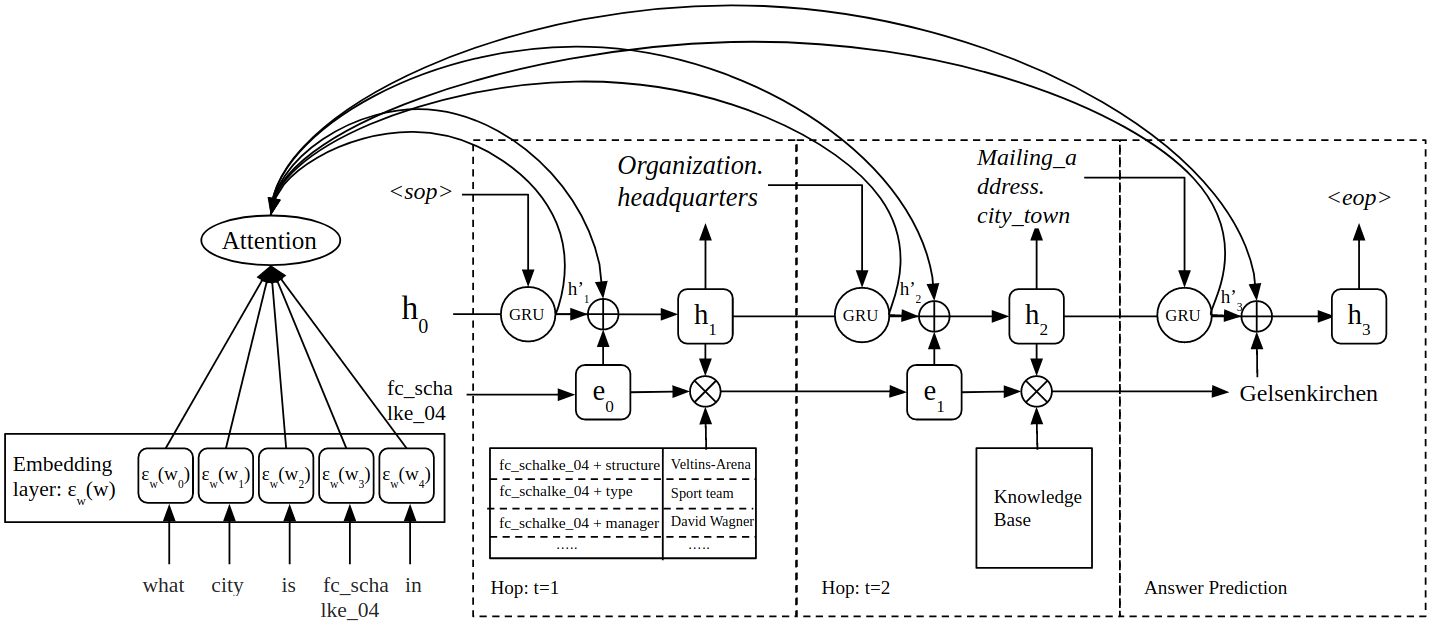
\includegraphics[width=1.0\columnwidth]{Images/model.png}
\caption{An illustration of how our model works with a QA pair \textit{``What city is fc\_schalke\_04 in?''} and \textit{Gelesenkirchen}. The entity linker extracts \textit{fc\_schalke\_04} as the topic entity. We only show one possible paths here: $r_1$ is \textit{Organization.headquarters} and $r_2$ is \textit{Mailing\_address.city\_town}, our model can be used to output the probability of this given path. The symbol $\bigoplus$ represents concatenation, and $\bigotimes$ represents knowledge base lookup. }
\label{fig:model}
\end{figure*}


We first introduce some notations. For a given question $q$ and its topic entity $e_0$ (identified by entity linking tool), a reasoning path is a sequence in the form $\mathbf{p} = (e_0, r_{1},e_{1},r_{2}, \cdots,e_{T-1}, r_{T})$ that points to the answer entity $e_T=y$. That is, $\mathbf{p}\rightarrow e_T=y$. Each step $(e_{t-1},r_t,e_t)$ is a valid fact in the knowledge base $\mathcal{KB}$. We assume that there are multiple valid paths $\mathbf{p}\in \mathcal{P}$ that can lead to the correct answer $y$ and they are not given by the annotator in the dataset. We treat these paths as hidden variables and we marginalize them out to compute the probability of getting the answer $y$:

\begin{align}
&p(y|q)\nonumber=\sum_{\mathbf{p}\in\mathcal{P}} [p(e_{T(\mathbf{p})}=y|\mathbf{p},q)p(\mathbf{p}|q)] \nonumber
=\sum_{\mathbf{p}\in\mathcal{P}}\prod_{t=1}^{T(\mathbf{p})} [p(e_t|e_{t-1},r_t) p(r_t|q,e_0,r_1,\cdots,e_{t-1})]
\label{eq:marginal}
\end{align}
where $\mathcal{P}$ is a set of all valid paths leading to the answer $y$, and $T(\mathbf{p})$ is the number of hops in the path $\mathbf{p}$.

Given this training objective, we want to calculate the value of two terms, $p(e_{T(\mathbf{p})}=y|\mathbf{p},q)$ and $p(\mathbf{p}|q)$. Solving the probability of latent variable $\mathbf{p}$ conditioned on $q$ can be seen as a sequence prediction task. Figure \ref{fig:model} illustrates the architecture of our model. We integrate the $\mathcal{KB}$ and the entity representations into the RNN model. At a timestep $t$, the input hidden representations of GRU unit and predicted relation are denoted by $h_{t-1}$ and $r_t$ respectively. The model relies on the attention mechanism~\cite{DBLP:journals/corr/BahdanauCB14} to produce a question context vector $c_t$. Specifically, all the words $w_0,w_1,\cdots,w_{|q|-1}$ in the given question $q$ are first sent to a fixed embedding layer to acquire word embeddings $\varepsilon_w(w_0),\varepsilon_w(w_1),\cdots,\varepsilon_w(w_{|q|-1})$. Next we apply GRU to produce a temporary hidden state $h_{t}'=GRU(h_{t-1}, r_{t-1})$, and then apply a parameterized feed-forward neural network $a$ to calculate the similarity score $u_{tk} = a(h'_{t},\varepsilon_w(w_k))$ of two inputs $h'_{t}$ and $\varepsilon_w(w_k)$, and then these scores are normalized into attention weights $\alpha_{tk}=\frac{\exp (u_{tk})}{\sum_{0\leq j\leq |q|-1}\exp (u_{tj})}$, which are used to produce the question context vector $c_t=\sum_{0\leq j\leq |q|-1}\alpha_{tj}\varepsilon_w(w_j)$. In this fashion, word embeddings are combined in different ways based on attention weights to show different reasoning focuses at each timestep.

The model then concatenates temporary hidden state $h_{t}'$, entity representation $\varepsilon_e(e_{t-1})$, and question context $c_t$ together, and passes the concatenation through a linear transformation $f$ with ReLU activation to obtain the hidden state $h_t=ReLU(f([h'_{t}; \varepsilon_e(e_{t-1}); c_t]))$. This process is recurrently done until the model predicts a stop symbol \textit{<eop>}\footnote{This stop mechanism is the same as how it works in a vanilla RNN. Similarly, we also attach <sop> to the beginning of each sequence to denote the start state. We will omit these symbols in formulas for simplicity.}. Note that the vanilla RNN attention model only has $h_{t}'$ and $c_t$ when calculates $h_t$. We add entity representation into the calculation, since entity captures important information in the reasoning path. The probability of predicting the $k$-th relation $\gamma_k$ in $\mathcal{R}$ at timestep $t$ is:
\begin{align*}
&p(r_t=\gamma_k|q,e_0,r_1,\cdots,e_{t-1})= \frac{\exp <h_t,\varepsilon_r(\gamma_k)>}{\sum_j\exp <h_t,\varepsilon_r(\gamma_j)>}
\end{align*}
where $\varepsilon_r$ is the embedding function, $<>$ is the dot product between two inputs.


Given the previous entity $e_{t-1}$ and relation $r_t$, the next matched entity may not be unique when we query the knowledge base. %(another way to collect this entity is via a soft lookup with a key-value memory network structure. We provide more details in the appendix.) 
For example, if $e_{t-1}$=``united states'', and $r_t=$ ``president of'', then the resulting entity has 45 possibilities. Since we do not have additional constraints, all of them are equally likely to be selected, and hence we define:
\begin{align}
  %&p(e_t|q,e_0,r_1,\cdots,e_{t-1},r_t)\\\nonumber
  %=&\;
  p(e_t|e_{t-1},r_t)
  =\begin{cases}
  1/M & \text{if }e_t\text{ is one of the }M\text{ matched entities} \\
  0 & \text{if }e_t\text{ is not a matched entity}
\end{cases} 
\end{align}

Thus the probability of a path containing both entities and relations can be computed using the chain rule:

\begin{align}
p(\mathbf{p}|q)\nonumber
= \prod_{t=1}^{T-1}p(e_t|e_{t-1},r_t)\prod_{t=1}^{T}p(r_t|q,e_0,r_1,\cdots,e_{t-1}) 
\end{align}

To train our model, we would like to maximize the answer probability $p(y|q)$ using only the given answer for each training instance. To make prediction on each test case, we would like to find the answer $y$ with the highest probability.

In order to train our model by maximizing the marginalized answer probability given in (\ref{eq:marginal}), it requires summing over all valid reasoning paths from the topic entity to the answer entity in knowledge base. To achieve this goal, we first apply depth first search (DFS) algorithm with maximum 3 hops to get valid path candidates. The algorithm starts the traversal from the topic entity node, and ends at the answer entity node. All possible paths between the topic entity and the answer entity within 3 hops are extracted as candidates. We then set a threshold to remove paths which point to too many entities at the last hop. Note that training with this algorithm does not require ground truth reasoning path label. Labeled reasoning path is a plus, but not necessary. If it is given, we can either include the ground truth paths in $\mathcal{P}$, or use them to initialize model training.

\begin{table}[t]
\centering
\resizebox{0.5\columnwidth}{!}{
\begin{tabular}{|l|c|c|}
\hline
              & WQSP & CWQ \\
\hline
STAGG\_SP \cite{DBLP:conf/acl/YihRMCS16} & 71.7 & -   \\
HR-BiLSTM \cite{DBLP:conf/acl/YuYHSXZ17}         & 62.3 & 31.2     \\
KBQA-GST \cite{DBLP:conf/ijcai/LanW019}     & 67.9 & 36.5   \\
\hline
KV-MemNN* \cite{DBLP:conf/emnlp/MillerFDKBW16}  & 38.6 & -   \\
STAGG\_answer* \cite{DBLP:conf/acl/YihRMCS16} & 66.8 & -   \\
NSM* \cite{DBLP:conf/acl/LiangBLFL17} & \textbf{69.0} & -   \\
GRAFT-Net* \cite{DBLP:conf/emnlp/SunDZMSC18}        & 62.8 & 26.0   \\

%Our Method-joint\_prob       &   62.1 &  38.0    \\
%Our Method-joint\_prob\_short       &   58.4 &      \\
%Our Method-joint\_prob\_random       &   58.8 &      \\
%Our Method-joint\_prob\_multiple\_paths       & 63.9   &   -    \\
%Our Method-marginal\_prob\_with\_true\_label       &  \textbf{68.5}  &    34.8   \\
Our Method-marginal\_prob*       &  67.9  &   \textbf{41.9}  \\
%Our Method-obj3+new\_decode &   &     \\
\hline
\end{tabular}
}
\caption{ We report F1 ($\%$) on WQSP and CWQ test sets. Methods labeled with $*$ only require the final answer as the supervision, and they are directly comparable to our model. As references, We also report the performance of methods that requires extra supervisions in the first block.}\label{tab:wqsp_cwq}
\end{table}

We conduct experiments on two multi-hop KBQA datasets, \textsc{WebQuestionSP} (WQSP) \cite{DBLP:conf/acl/YihCHG15}, \textsc{ComplexWebQuestion}-1.1 (CWQ) \cite{DBLP:journals/corr/abs-1807-09623}, and use the original train/dev/test split. In Table \ref{tab:wqsp_cwq} we compare our method to state-of-the-art models. All comparisons are divided into two groups based on different training supervisions. The upper block shows methods that are only trained with final answer as supervision, and the second block contains methods using extra annotations such as parsing results of the query. Experimental results show that our model performs better than all other methods on two datasets except for NSM \cite{DBLP:conf/acl/LiangBLFL17} on WQSP. Although NSM only relies on answers to train their model, it requires many prior knowledges, such as a big vocabulary to train word embeddings and graph embeddings, type label of the entity and of the relation, and pre-defined templates. The experiments from their papers show that these knowledge play a very important role in the system, \emph{e.g.} F1 score drops from 69.0 to 60.7 by not using the pretrained embeddings. %In contrast, our model supports a training method that takes only raw QA pairs and the facts in knowledge base, and does not rely on any additional labels and pre-defined knowledge. 
 Also, NSM is only tested on a single dataset, \emph{i.e.} WQSP. It is unclear whether they could perform consistently well on different datasets. Among all the methods, \textsc{STAGG} performs the best when additional annotation is provided, but we can see a clear drop between \textsc{STAGG\_SP} and \textsc{STAGG\_answer} when such annotation is not available.

%By comparing performance of using different objectives as shown in the second block of the table, we can see that there is a significant improvement by considering multiple relation paths in training. The performance gap between joint objective and marginal objective demonstrates that our proposed marginal objective is a much better way to train a model with multiple relation paths. We do not observe a very different results by using or not using labeled relation paths, which is a good signal. 




%To further disentangle the contribution of different factors in our method, we present a feature ablation test on WQSP dataset shown in Table \ref{tab:wqsp_cwq_ablation}. The vanilla RNN structure only maintains a hidden state and the previous prediction in the loop. Here, we show the performance boost by considering entity features in KBQA task. Instead of using greedy algorithm or beam search to output the top prediction with the highest joint probability $P(y,\mathbf{p})$, we propose to make the prediction based on marginalized probability $P(y)$, which also improves the performance by $1.8\%$.


\section{Proposed Work}


    
\subsection{Handling Noisy Tags in Multi-label Classification}  \label{future_noise}

When we collected data from TheGuardian and Slashdot websites, we also gathered a list of user tags\footnote{\scriptsize\url{www.zubiaga.org/datasets/socialbm0311/}} for each document, and treated them as additional features in the multi-label prediction experiments. These user tags are labeled by humans as bookmarks of the webpage. For example, a document is labeled with \texttt{world\_news}, \texttt{africa}, \texttt{somalia}, \texttt{water\_tra\\nsport}, and \texttt{piracy\_at\_sea} in the TheGuardian, and the corresponding user tags are \texttt{history}, \texttt{piracy}, \texttt{historia}, \texttt{somalia}, \texttt{pirate}, \texttt{somali}, \texttt{nmm}, and \texttt{piratería}. Given both clean tags and user tags, we can build a dataset labeled with two groups of tags, where the clean tags can be viewed as ground truth labels and the user tags can be viewed as noisy annotations which contain both useful information and noises. In this way, we have three exclusive sets in the dataset, a set labeled with only clean tags, a set labeled with only noisy tags, and a set labeled with both clean and noisy tags. The goal is to train a classifier to solve the multi-label task by using all three sets.

Most existing investigations use non-practical simulated approaches to evaluate their method on learning from label noise. People inject label noises based on some controlled and known corruption process to a clean dataset (e.g. assuming label noise is uniformly distributed among all categories, and flipping the label of each category based on the distribution.) \cite{zhang2018generalized,tanaka2018joint,yi2019probabilistic}. In contrast, our datasets reflect the practical setup: (1) Our datasets contain real-world label noise collected from bookmark sharing sites. (2) The noisy annotations and clean annotations do not use consistent vocabulary, which means that a noisy tag may never show up in the clean training set. Existing approaches can be classified into two groups: learning to map clean labels to noisy labels \cite{sukhbaatar2014learning2,sukhbaatar2014training2,goldberger2016training2}, and learning to map noisy labels to clean labels\cite{dehghani2017fidelity2,wu2018light,yuan2018iterative}. To map clean labels to noisy labels, one can add an additional prediction layer on top of the output layer of a standard classifier. In this way, the clean label is built as latent variable in the model, and predicted in the middle of the learning process. One needs to estimate the value of latent variable to solve a task with noisy tags as the final supervision. To map noisy labels to clean labels, one can train a separate classifier on the samples which have both noisy labels and clean labels. And this additional classifier can be used to map all noisy labels back to clean labels. After cleaning the dataset, a regular supervised learning method can be plugged in to solve the task.



\subsection{Relation Path Selection in KBQA}  \label{future_path}

In KBQA task, DFS algorithm can generate a large number of paths starting from the topic entity and ending at the correct answer, but not all of them are good training samples for a machine learning model. A research task would be to distinguish good training samples from bad training samples. As the example shown in Figure \ref{QAPaths}, there are four paths ($\mathbf{p}^1$,$\mathbf{p}^2$,$\mathbf{p}^3$,$\mathbf{p}^4$) pointing to the exact answer set containing only the answer entity, and thus can be treated as ground truth paths when training. Comparatively, reasoning paths $\mathbf{p}^5$ and $\mathbf{p}^6$ lead to a larger final entity set containing the correct answer \textit{``West Lafayette''} but also other entities. These two paths can be considered as inferior to the top 4 paths; however, it is still worth including them in the training as a ``second choice'', as it is not difficult to extract the correct answer from final sets by additional post-processing. For example, a simple filter can be applied to filter out \textit{``United States of America''} and \textit{``Indiana''} from the predicted set, as they are not cities. Path $\mathbf{p}^7$ is bad because it is not interpretable, in addition to the final answer set being exaggeratedly large with invalid answers. Hence, path $\mathbf{p}^7$ should not be considered as a training path for this question. %Unfortunately, it is not possible for any existing models to use multiple good/inferior paths, but not the bad ones, since current models are only trained with a single path for each question answer pair.

To improve the current model, we want the model to not only output diverse reasoning paths, but also reward the ``better'' paths over the inferior ones by assigning ``better'' paths higher probabilities. For example, $R_5, R_6, R_7$ in Figure \ref{QAPaths} are not very helpful for training, thus should receive low probabilities in the prediction process, and be removed from training. In this proposed work, we can follow the idea used in multi-label prediction task to use the current trained model to weight the importance of each path, and filter out paths assigned with low importance. Specifically, we can train a model based on all paths generated by DFS algorithm first. After a few epochs, we stop training and use the trained model to assign probabilities to each path. The model can select useful paths by dynamically choosing reasoning paths deemed as most probable by the current model during training. The overall training procedure can be summarized in Algorithm \ref{alg:train}. All the notations used here are the same as them in section \ref{path_nota}. 


\begin{algorithm}
 \SetKwInOut{Input}{Input}
 \SetKwInOut{Output}{Output}

 % \underline{function Euclid} $(a,b)$\;
 \Input{KBQA dataset $(q^{n},y^{n}, e_0^{n}),n=1,2,\cdots,N$, \\
 Knowledge Base $\mathcal{KB}$, \\
 Threshold $k_1$ and $k_2$. }
 \Output{Trained model parameters}
 \ForEach{instance $(q^{n},y^{n}, e_0^{n})$}{Use DFS algorithm to get a set of paths $\mathcal{P}^n$ from $e_0^{n}$ to $y^{n}$.\\
 Remove from $\mathcal{P}^n$ paths that point to more than $k_1$ entities.\\}
 
 % Initialize model parameters\\
 \ForEach {batch}{
 % \ForEach {batch }{
  \ForEach{$(q^{n},y^{n}, e_0^{n})$ in the batch}{
  Get top $k_2$ paths in $\mathcal{P}$ sorted by $p(\mathbf{p}|q)$ based on current model:
		 	$\tilde{\mathcal{P}}^n = \{{\mathbf{p}}^n_{1},\cdots,{\mathbf{p}}^n_{k_2} \}$\\
  } 
    Update model parameters by maximizing $\sum\limits_{(q^{n},y^{n}, e_0^{n}) \in \text{batch}} \log \sum\limits_{\mathbf{p} \in \tilde{\mathcal{P}}^n} p(y^{n}|\mathbf{p},q^{n}) P(\mathbf{p}|q^{n}) $
  }

 \caption{Our training method}
 \label{alg:train}
\end{algorithm}

In addition, the other goal of filtering out bad paths is to remove bad reasoning paths which are not relevant to the query. For example, a sample question from WQSP is \textit{who was the owner of kfc?}, the graph search algorithm can easily extract two ``correct'' paths starting from the topic entity \textit{kfc} directing to the ground truth answer \textit{Colonel Sanders}: \textit{kfc $\rightarrow$ organization.organization.founders $\rightarrow$ Colonel Sanders} and \textit{kfc $\rightarrow$\ advertisingcharacters.product.advertising\_characters $\rightarrow$ Colonel Sanders}. However, the second path is totally wrong given that the reasoning path is irrelevant to the given question. \textit{Colonel Sanders} happens to be the advertising character of \textit{kfc}, but this cannot be generalized to other cases. Without using the trained model to filter out this irreverent path, the model may learn incorrect map from \textit{who is the owner...} to the relation \textit{advertising\_characters}.

Furthermore, this path selection task can also be associated with the task that handles noisy samples introduced in the previous subsection. DFS algorithm returns us both informative and bad paths. Bad paths can be seen as noises in the training set, and hurt the model performance. Reed \cite{reed2014training2} proposed a bootstrapping approach to train a model with noises included in the training set. Their idea is similar to the one proposed here - using trained model to distinguish clean samples from noisy samples. Follow-up work proposes different variants of bootstrapping methods by using pre-defined knowledge and advanced model structures \cite{tanaka2018joint,yi2019probabilistic,han2019deep}. All these existing work can be considered as baselines in our experiment.


\subsection{Model Architecture} \label{future_model}

We also propose to use different sequence model structures in sequence prediction task. For example, in KBQA task, we are given a knowledge graph as important context information. In our current model, the knowledge graph is stored in a dictionary, where the key is head entity and the value is the concatenation of relation and tail entity (e.g. \{``United States'' : [``president'', ``Donald Trump'']\}). A future research topic would be to find the best way to store knowledge graph and integrate it into the sequence prediction model. Now we just simply use a dictionary lookup function to extract information from the knowledge graph. In the future, we would like to construct a memory matrix to store knowledge base, similar to~\cite{DBLP:conf/emnlp/MillerFDKBW16}. Each memory slot is a key-value pair to denote a fact in the knowledge base, where the key $k=[\varepsilon_e(e_{head});\varepsilon_r(r_{mid})]$ is a vector representation which composed of the embeddings of head entity (subject) and the relation, and the value $v=\varepsilon_e(e_{tail})$ is a vector representation of the tail entity (object). Both relation and entity embeddings are pre-trained and not updated by our model. The following graph embedding methods will be considered: \textsc{Word2vec} \cite{DBLP:journals/corr/abs-1301-3781}, \textsc{TransE} \cite{DBLP:conf/nips/BordesUGWY13}, and \textsc{HolE} \cite{DBLP:journals/corr/TrouillonN17}. Similar to Key-value memory networks, our entity lookup module would involve the following steps: 

(1) Key hashing and addressing: in our model, predicted relation $r$ can be viewed as topic of the sub-question and used to pre-select a list of candidate $\mathcal{KB}$ facts. This operation can dramatically reduce the search space of the following matching process. It is done by filtering out memory slots where their keys do not contain $r$ ($\emph{i.e.}\ r_{mid}\neq r$). Each remaining memory slot is then assigned a relevance score $\beta$ by comparing its key with representations of previous entity and current relation: %$s_0$ is the embedding of the topic entity labeled by an entity linker tool.
\begin{align}
z_{tj} = b(h_t, k_j)
\end{align}
\vspace{-3ex}
\begin{align}
\beta_{tj} = \frac{\exp (z_{tj})}{\sum_i\exp (z_{ti})}
\end{align}

where $h_t$ is the vector representation of the hidden state in RNN, and $b$ is a parameterized feed-forward neural network used to measure the similarity between two inputs. 
% $\beta$ is a normalized score to represent relevance.

(2) Value reading: the values of memories are read by taking their weighted sum using the relevance scores.
\begin{align}
s_t =\sum_{i}\beta_{ti}v_i
\end{align}

where $s_t$ is the representation of the predicted entity. This entity lookup step can be viewed as executing a query in embedding space. The model use a head entity and a relation to search for the object from the memory, and the output $s$ can be viewed as the representation of the searching result. This step can also interpreted as a soft style entity lookup by assigning attention on all memory keys compared to the current hard style dictionary lookup method.